\begin{marginfigure}
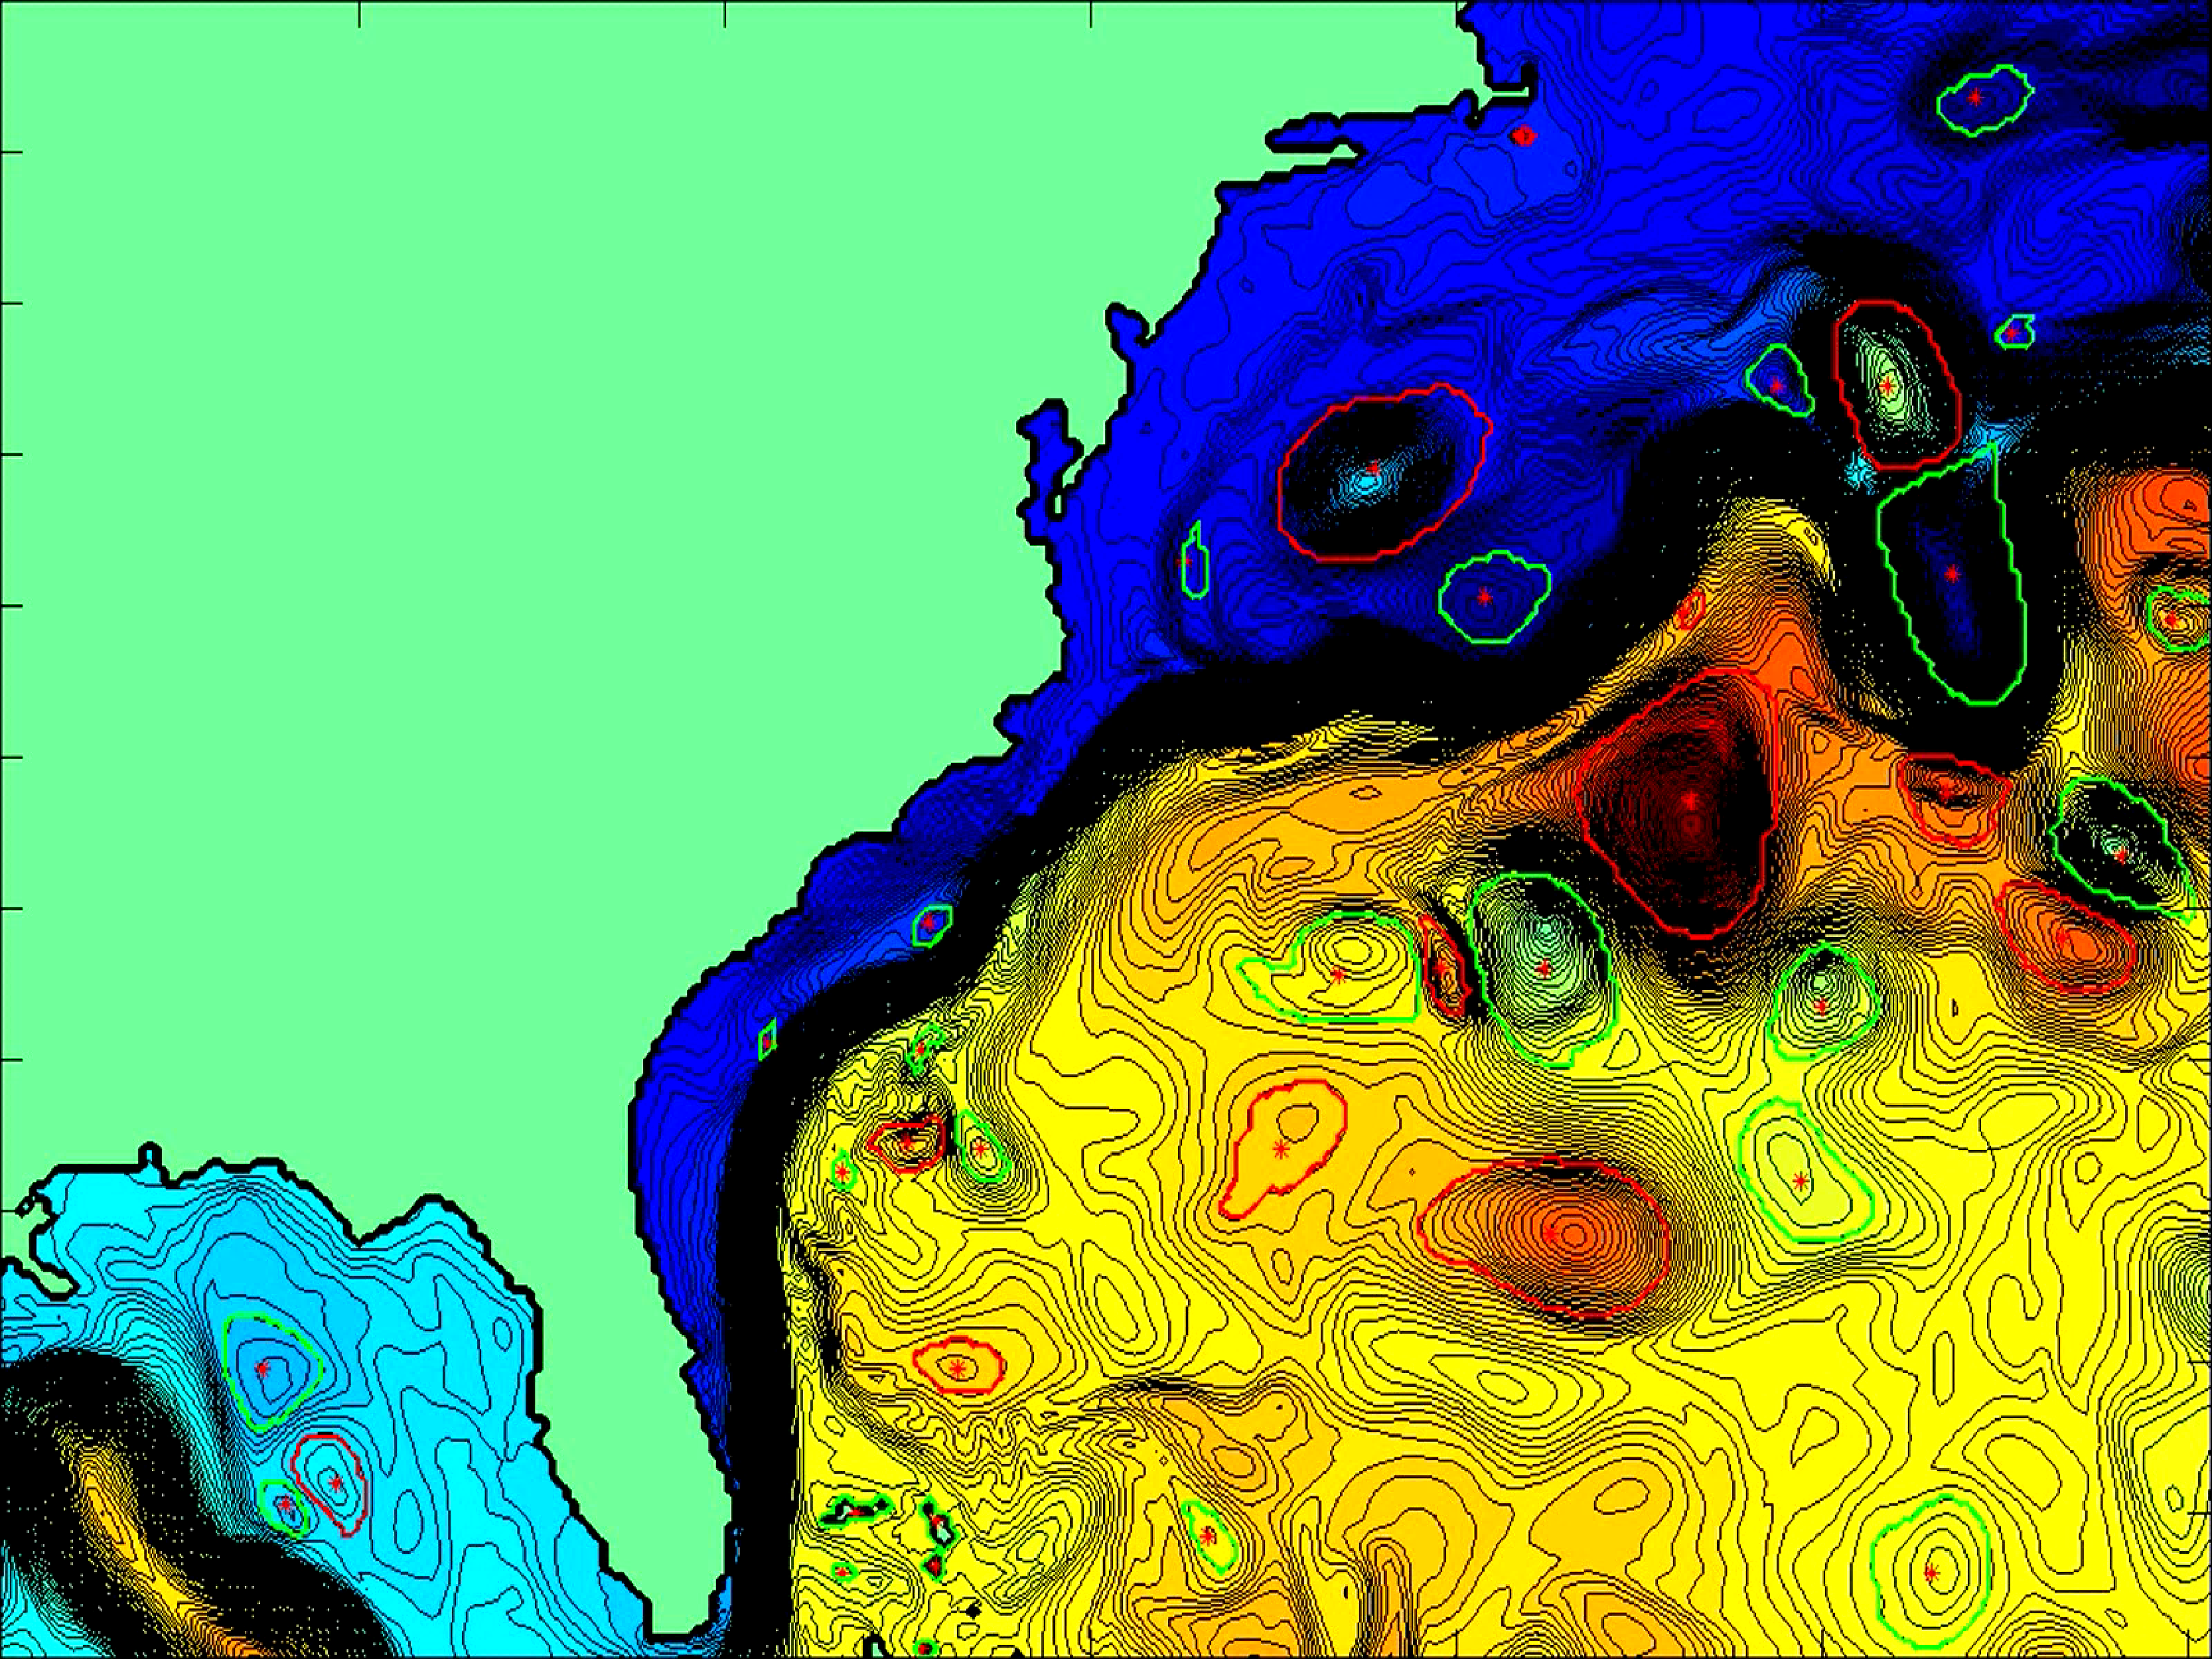
\includegraphics[]{GS.pdf}
\caption{Animation snapshot of early test run. Shown is \SSH~with detected eddies indicated by red and green lines.}
\end{marginfigure}

%\newthought{This } section discusses the theory of meso-scale turbulence and parametrizations thereof.
\newthought{Geostrophic } turbulence is typically characterized by rather stable, often deep reaching, more or less circular, coherent pressure anomalies that rotate fluid around in a vortex in quasi-geostrophic equilibrium \citep{Zhang2013}. These entities can persist for long periods of time in which they often travel distances on the order of hundreds of kilometers
zonally. The fact that baroclinic instability leads to these vortices, instead of cascading to ever smaller scales as would be expected from chaotic
turbulence, is a direct consequence of the inverse energy cascade of two-dimensional motion\footnote{For a discussion of this phenomenon see~\cref{chap:turbu_categories}.} (see~\cref{fig:PSI}.) \citep{Rhines1979,Meneguzzis1988}.
The atmospheric analog are storms and high-pressure systems, yet with much less difference between high- and low-pressure systems in the ocean due to
a smaller centrifugal force \ie smaller Rossby number ($\Ro$). These quasi-geostrophic, mesoscale vortices \ie \textit{eddies}\footnote{For a discussion of the different types of vortices in the ocean see \cref{appendix:eddy_cat}.}, are readily visible on \SSH-maps (see~\cref{fig:SSHB}). Yet, it is difficult to \emph{define} an eddy in terms of physical variables. The transition from meandering jet or other undeveloped
baroclinic turbulence to a coherent vortex is not very sharp. Eddies also sometimes merge or split or collectively form rifts and valleys in \SSH. Detecting them on one snapshot automatically via an algorithm is therefore not trivial. Further complications arise when the algorithm is also supposed to track each individual eddy over time. Their sheer abundance at any
given point in time inevitably creates ambiguities  as to \textit{which is which} between time steps.

\newthought{From}~the automated-tracking censuses that have thus far been presented (\citet{Chelton2011,Chelton2007,Petersen2013}) and from the numerous publications of investigations into geostrophic scales and phase speeds via satellite \SSH~products by other means (\eg spectral methods, \citep{scott2005direct,Chelton2011,Stammer1997}) it appears that results critically depend on the resolution of the particular \SSH~product used and/or the methods by which said parameters were derived, as scales, phase speeds and other parameters generally do not agree very well among the different publications. Comparison to theory is usually also rather unsatisfactory which should come as no surprise since the physics of non-linear eddies are still far from complete so that results can usually only be compared to linear theory. 

\newthought{The}~main questions that motivated this work therefor are:
\begin{enumerate}
\setlength\itemsep{1mm}
\item
How should an eddy be \textit{defined} and how should this understanding be implemented in the algorithm? Do the different approaches affect the results?
\item
Is it possible to derive realistic horizontal eddy scales from satellite altimetry products via an automated \SSH-based eddy-census. How should such scale be defined and is the resolution in time and space of the \avi~product sufficient for precise determinations? What are those scales?   
\item
Is it possible to automatically track eddies and use those tracks to derive eddy drift vectors? How reliable is the tracking and to what extent is its quality influenced by resolution in time? How do the zonal drift speeds compare to theory? 
\item
How do scales and drift speeds derived from satellite \SSH~compare to those derived from eddy-resolving ocean model \SSH?
\end{enumerate}
